\documentclass[a4paper,11pt]{article}
\usepackage[polish]{babel}
\usepackage[utf8]{inputenc}
\usepackage[T1]{fontenc}
\usepackage{graphicx}
\usepackage{anysize}
\usepackage{xcolor}
\usepackage{mdframed}
\usepackage{float}

\sloppy

\begin{document}

\section*{Całka Riemanna}

Niech dana będzie funkcja ograniczona $f \colon [a, b] \to \mathbb{R}$. Sumą częściową (Riemanna) nazywa się liczbę 

$$ \mathbf{R}_{f,P(q_1, \dots q_n)} = \sum^{n}_{i=1} f (q_i) \cdot \Delta p_i .$$

Funkcję $f$  nazywa się całkowalną w sensie Riemanna lub krótko R-całkowalną, jeśli dla dowolnego ciągu normalnego $(P^k)$ podziałów przedziału $[a,b]$, istnieje (niezależna od wyboru punktów pośrednich) granica 

$$ \mathbf{R}_f = \lim_{k \to \infty} \mathbf{R}_{f,P^k (q_1^k, \dots , q^k_{n_k})}$$

nazywana wtedy całką Riemanna tej funkcji. Równoważnie: jeżeli istnieje taka liczba $\mathbf{R}_f$, że dla dowolnej liczby rzeczywistej $\varepsilon > 0$ istnieje taka liczba rzeczywista $\delta >0 $, że dla dowolnego podziału $P (q_1, \dots , q_n)$ o średnicy \textbf{diam} $ P(q_1, \dots , q_n) < \delta$; bądź też w języku rozdrobnień: że dla dowolnej liczby rzeczywistej $\varepsilon > 0$ istnieje taki podział $S(t_{1},\dots ,t_{m})$ 
przedziału $[a,b]$, że dla każdego podziału $ P(q_{1},\dots ,q_{n})$ rozdrabniającego $ S(t_{1},\dots ,t_{m})$  zachodzi

$$\left| R_{{f,P(q_{1},\dots ,q_{n})}}-R_{f}\right|<\varepsilon .$$


Funkcję $f$ nazywa się wtedy całkowalną w sensie \textsc{\textit{Riemanna}}  (R-\textit{całkowalną}), a liczbę $R_{f}$ jej \textbf{całką Riemanna}.



\begin{figure}[htb]
\begin{mdframed}[backgroundcolor=red!20]
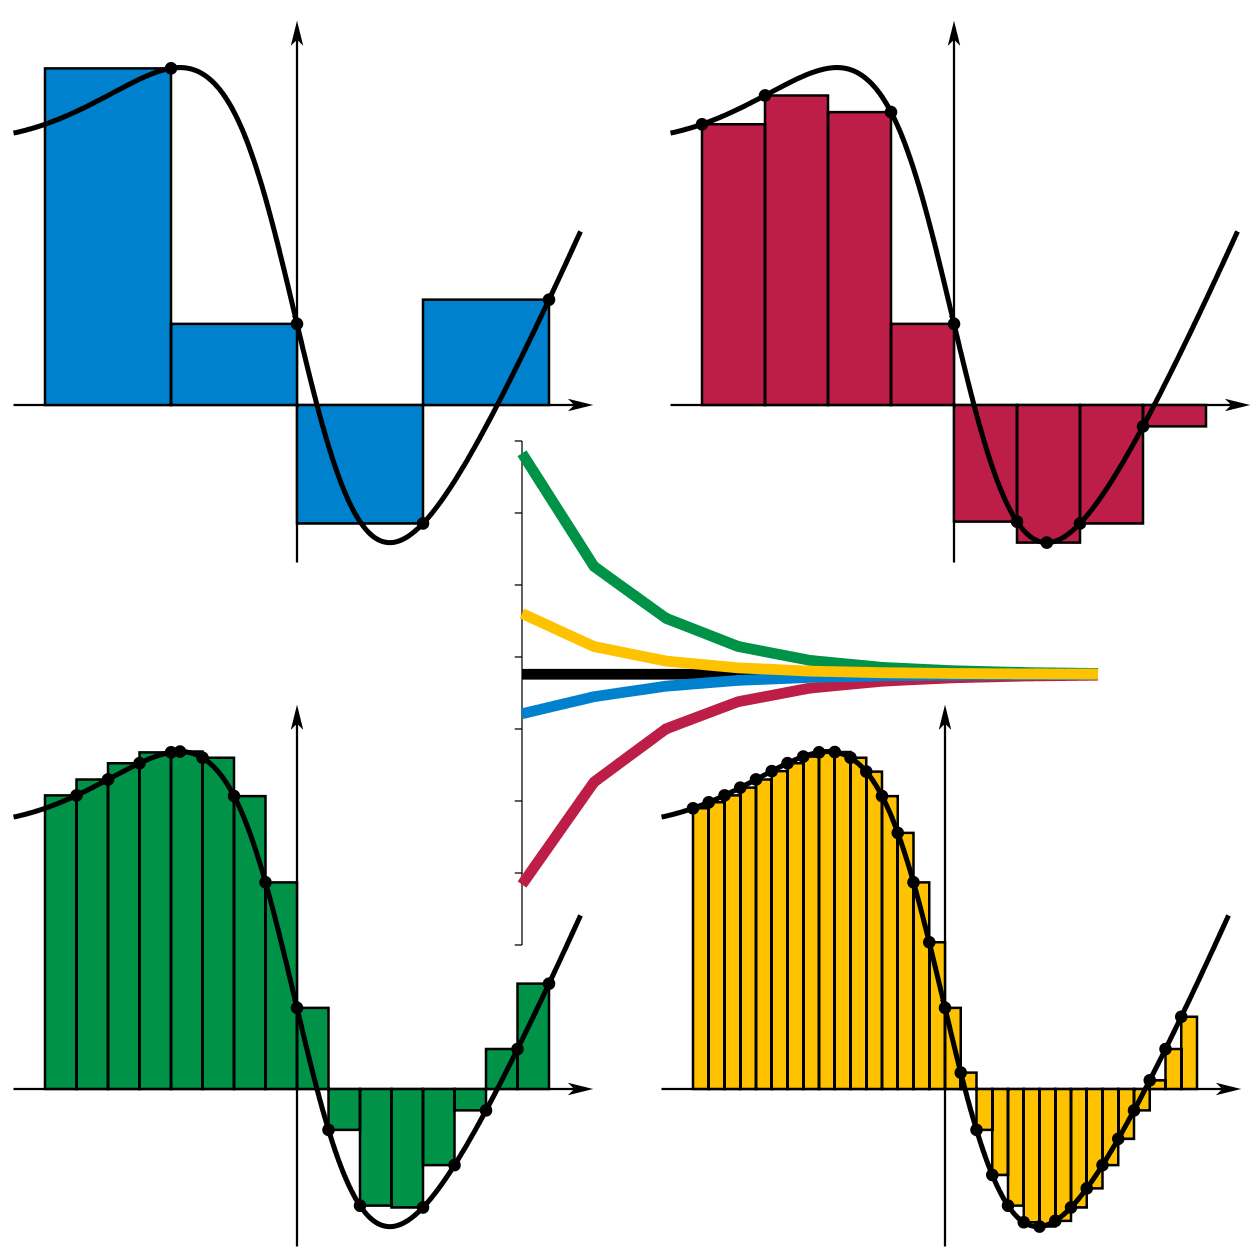
\includegraphics[scale=0.5]{Riemann_sum_convergence.png}

Przykład sum Riemanna przy wyborze punktu pośredniego w prawym końcu podprzedziału (niebieski), w wartości minimalnej (czerwony) i maksymalnej (zielony) funkcji w podprzedziale i lewego końca podprzedziału (żółty). Wartość wszystkich czterech przypadków zbliża się do 3,76 przy powiększaniu liczby podprzedziałów od 2 do 10 (w domyśle, również nieograniczenie).
\end{mdframed}
\label{fig:pic}
\end{figure}





\end{document}
